% Options for packages loaded elsewhere
\PassOptionsToPackage{unicode}{hyperref}
\PassOptionsToPackage{hyphens}{url}
%
\documentclass[
]{book}
\usepackage{lmodern}
\usepackage{amsmath}
\usepackage{ifxetex,ifluatex}
\ifnum 0\ifxetex 1\fi\ifluatex 1\fi=0 % if pdftex
  \usepackage[T1]{fontenc}
  \usepackage[utf8]{inputenc}
  \usepackage{textcomp} % provide euro and other symbols
  \usepackage{amssymb}
\else % if luatex or xetex
  \usepackage{unicode-math}
  \defaultfontfeatures{Scale=MatchLowercase}
  \defaultfontfeatures[\rmfamily]{Ligatures=TeX,Scale=1}
\fi
% Use upquote if available, for straight quotes in verbatim environments
\IfFileExists{upquote.sty}{\usepackage{upquote}}{}
\IfFileExists{microtype.sty}{% use microtype if available
  \usepackage[]{microtype}
  \UseMicrotypeSet[protrusion]{basicmath} % disable protrusion for tt fonts
}{}
\makeatletter
\@ifundefined{KOMAClassName}{% if non-KOMA class
  \IfFileExists{parskip.sty}{%
    \usepackage{parskip}
  }{% else
    \setlength{\parindent}{0pt}
    \setlength{\parskip}{6pt plus 2pt minus 1pt}}
}{% if KOMA class
  \KOMAoptions{parskip=half}}
\makeatother
\usepackage{xcolor}
\IfFileExists{xurl.sty}{\usepackage{xurl}}{} % add URL line breaks if available
\IfFileExists{bookmark.sty}{\usepackage{bookmark}}{\usepackage{hyperref}}
\hypersetup{
  pdftitle={Guía de Economía Aplicada Sectorial},
  pdfauthor={Francisco Fernández},
  hidelinks,
  pdfcreator={LaTeX via pandoc}}
\urlstyle{same} % disable monospaced font for URLs
\usepackage{color}
\usepackage{fancyvrb}
\newcommand{\VerbBar}{|}
\newcommand{\VERB}{\Verb[commandchars=\\\{\}]}
\DefineVerbatimEnvironment{Highlighting}{Verbatim}{commandchars=\\\{\}}
% Add ',fontsize=\small' for more characters per line
\usepackage{framed}
\definecolor{shadecolor}{RGB}{248,248,248}
\newenvironment{Shaded}{\begin{snugshade}}{\end{snugshade}}
\newcommand{\AlertTok}[1]{\textcolor[rgb]{0.94,0.16,0.16}{#1}}
\newcommand{\AnnotationTok}[1]{\textcolor[rgb]{0.56,0.35,0.01}{\textbf{\textit{#1}}}}
\newcommand{\AttributeTok}[1]{\textcolor[rgb]{0.77,0.63,0.00}{#1}}
\newcommand{\BaseNTok}[1]{\textcolor[rgb]{0.00,0.00,0.81}{#1}}
\newcommand{\BuiltInTok}[1]{#1}
\newcommand{\CharTok}[1]{\textcolor[rgb]{0.31,0.60,0.02}{#1}}
\newcommand{\CommentTok}[1]{\textcolor[rgb]{0.56,0.35,0.01}{\textit{#1}}}
\newcommand{\CommentVarTok}[1]{\textcolor[rgb]{0.56,0.35,0.01}{\textbf{\textit{#1}}}}
\newcommand{\ConstantTok}[1]{\textcolor[rgb]{0.00,0.00,0.00}{#1}}
\newcommand{\ControlFlowTok}[1]{\textcolor[rgb]{0.13,0.29,0.53}{\textbf{#1}}}
\newcommand{\DataTypeTok}[1]{\textcolor[rgb]{0.13,0.29,0.53}{#1}}
\newcommand{\DecValTok}[1]{\textcolor[rgb]{0.00,0.00,0.81}{#1}}
\newcommand{\DocumentationTok}[1]{\textcolor[rgb]{0.56,0.35,0.01}{\textbf{\textit{#1}}}}
\newcommand{\ErrorTok}[1]{\textcolor[rgb]{0.64,0.00,0.00}{\textbf{#1}}}
\newcommand{\ExtensionTok}[1]{#1}
\newcommand{\FloatTok}[1]{\textcolor[rgb]{0.00,0.00,0.81}{#1}}
\newcommand{\FunctionTok}[1]{\textcolor[rgb]{0.00,0.00,0.00}{#1}}
\newcommand{\ImportTok}[1]{#1}
\newcommand{\InformationTok}[1]{\textcolor[rgb]{0.56,0.35,0.01}{\textbf{\textit{#1}}}}
\newcommand{\KeywordTok}[1]{\textcolor[rgb]{0.13,0.29,0.53}{\textbf{#1}}}
\newcommand{\NormalTok}[1]{#1}
\newcommand{\OperatorTok}[1]{\textcolor[rgb]{0.81,0.36,0.00}{\textbf{#1}}}
\newcommand{\OtherTok}[1]{\textcolor[rgb]{0.56,0.35,0.01}{#1}}
\newcommand{\PreprocessorTok}[1]{\textcolor[rgb]{0.56,0.35,0.01}{\textit{#1}}}
\newcommand{\RegionMarkerTok}[1]{#1}
\newcommand{\SpecialCharTok}[1]{\textcolor[rgb]{0.00,0.00,0.00}{#1}}
\newcommand{\SpecialStringTok}[1]{\textcolor[rgb]{0.31,0.60,0.02}{#1}}
\newcommand{\StringTok}[1]{\textcolor[rgb]{0.31,0.60,0.02}{#1}}
\newcommand{\VariableTok}[1]{\textcolor[rgb]{0.00,0.00,0.00}{#1}}
\newcommand{\VerbatimStringTok}[1]{\textcolor[rgb]{0.31,0.60,0.02}{#1}}
\newcommand{\WarningTok}[1]{\textcolor[rgb]{0.56,0.35,0.01}{\textbf{\textit{#1}}}}
\usepackage{longtable,booktabs}
\usepackage{calc} % for calculating minipage widths
% Correct order of tables after \paragraph or \subparagraph
\usepackage{etoolbox}
\makeatletter
\patchcmd\longtable{\par}{\if@noskipsec\mbox{}\fi\par}{}{}
\makeatother
% Allow footnotes in longtable head/foot
\IfFileExists{footnotehyper.sty}{\usepackage{footnotehyper}}{\usepackage{footnote}}
\makesavenoteenv{longtable}
\usepackage{graphicx}
\makeatletter
\def\maxwidth{\ifdim\Gin@nat@width>\linewidth\linewidth\else\Gin@nat@width\fi}
\def\maxheight{\ifdim\Gin@nat@height>\textheight\textheight\else\Gin@nat@height\fi}
\makeatother
% Scale images if necessary, so that they will not overflow the page
% margins by default, and it is still possible to overwrite the defaults
% using explicit options in \includegraphics[width, height, ...]{}
\setkeys{Gin}{width=\maxwidth,height=\maxheight,keepaspectratio}
% Set default figure placement to htbp
\makeatletter
\def\fps@figure{htbp}
\makeatother
\setlength{\emergencystretch}{3em} % prevent overfull lines
\providecommand{\tightlist}{%
  \setlength{\itemsep}{0pt}\setlength{\parskip}{0pt}}
\setcounter{secnumdepth}{5}
\documentclass[12pt,a4paper,oneside]{article}
\begin{document}
$body$
\end{document}
\ifluatex
  \usepackage{selnolig}  % disable illegal ligatures
\fi
\newlength{\cslhangindent}
\setlength{\cslhangindent}{1.5em}
\newlength{\csllabelwidth}
\setlength{\csllabelwidth}{3em}
\newenvironment{CSLReferences}[2] % #1 hanging-ident, #2 entry spacing
 {% don't indent paragraphs
  \setlength{\parindent}{0pt}
  % turn on hanging indent if param 1 is 1
  \ifodd #1 \everypar{\setlength{\hangindent}{\cslhangindent}}\ignorespaces\fi
  % set entry spacing
  \ifnum #2 > 0
  \setlength{\parskip}{#2\baselineskip}
  \fi
 }%
 {}
\usepackage{calc}
\newcommand{\CSLBlock}[1]{#1\hfill\break}
\newcommand{\CSLLeftMargin}[1]{\parbox[t]{\csllabelwidth}{#1}}
\newcommand{\CSLRightInline}[1]{\parbox[t]{\linewidth - \csllabelwidth}{#1}\break}
\newcommand{\CSLIndent}[1]{\hspace{\cslhangindent}#1}

\title{Guía de Economía Aplicada Sectorial}
\author{Francisco Fernández}
\date{2021-02-12}

\begin{document}
\maketitle

{
\setcounter{tocdepth}{1}
\tableofcontents
}
\hypertarget{bienvenidos}{%
\chapter*{Bienvenidos}\label{bienvenidos}}
\addcontentsline{toc}{chapter}{Bienvenidos}

La presente Guía tiene el objetivo de proporcionar a los estudiantes de \textbf{Economía Aplicada Sectorial (AGRG-1001)} de la \href{https://www.umayor.cl/um/carreras/agronomia-santiago/10000}{\textbf{Escuela de Agronomía de la Universidad Mayor}} una guía de apoyo para la asignatura durante todo el semestre de este año. A través de esta guía tendrán acceso completo a toda el material que veremos durante el semestre y adicionalmente podrán poner en práctica todo lo que acá veamos.

El objetivo de la asignatura será entregar a los estudiantes una introducción sistemática a los conceptos y temas básicos de la economía en su relación con la agricultura en diferentes naciones, dando especial énfasis a la agricultura chilena. Para alcanzar este objetivo deberemos comprender las fuerzas macro y microeconómicas que influyen en las decisiones de productores y consumidores de la industrial alimentaria.

\hypertarget{U1}{%
\chapter{Introducción a la Economía Agraria}\label{U1}}

La presente unidad busca responder a las preguntas \emph{``¿Qué es la economía agraria?''} y \emph{¿Qué hace un economista agrario?}. En la primera sección, definiremos el alcance de la economía y conceptos claves para su definición, tales como recursos escasos, agentes económicos, trade-offs y costo oportunidad. De esta manera definiremos el campo de la economía y luego desarrollaremos nuestra definición de \textbf{Economía Agraria} basada en el papel que desempeñan los economistas agrarios a nivel micro y macro. La sección 2 proporciona antecedentes que permiten analizar la estructura cambiante de la agricultura mundial y nacional. Así mismo se establece la complejidad del sector agrario y su vínculo con un sin número de sectores.

\hypertarget{Sec1}{%
\section*{Sección 1: ¿Qué es la Economía Agraria?}\label{Sec1}}
\addcontentsline{toc}{section}{Sección 1: ¿Qué es la Economía Agraria?}

La Agricultura ha sido y continúa siendo uno de los sectores económicos más destacados de cualquier economía. \textbf{{[}Describir la importancia{]}}. En este curso particular nos focalizaremos en las relaciones económicas inherentes al sector agrícola.

Tomado en cuenta lo anterior, si contestaran a la pregunta \emph{¿Qué es la economía agraria?} definiéndola como ``la aplicación de principios económicos a la agricultura,'' estarían técnicamente en lo correcto, pero en un contexto limitado. Esta definición no reconoce los problemas económicos, sociales y ambientales que aborda la profesión de la economía agraria. Sería incorrecto percibir que esta se limita únicamente a la economía de las operaciones agrícolas y ganaderas. Estas operaciones representan anualmente alrededor del \href{https://www.worldbank.org/en/topic/agriculture/overview}{4\% del producto interno bruto (PIB) global}. Sin embargo, el alcance de la economía agraria va mucho más allá de la puerta del predio o explotación, abarcando una gama más amplia de actividades relacionadas con la industria alimentaria. En efecto, si ponemos como ejemplo a la agricultura chilena, el PIB de la actividad agropecuaria nacional puede pasar de un 2.93\% a un 14.36\% considerando la interacción del sector primario con la cadena agroalimentaria y procesamiento (lo que conoceremos como PIB ampliado) (\href{https://www.odepa.gob.cl/wp-content/uploads/2019/09/panorama2019Final.pdf}{Odepa, 2019}).

De esta manera, para obtener una mejor definición de \emph{economía agraria}, examinaremos primero el alcance de la economía y el papel que juegan los economistas agrícolas en la economía actual. Este examen nos permitirá proponer una respuesta más definitiva a la pregunta \emph{¿Qué es la economía agraria?}

\hypertarget{alcance-de-la-economuxeda}{%
\subsection*{Alcance de la Economía}\label{alcance-de-la-economuxeda}}
\addcontentsline{toc}{subsection}{Alcance de la Economía}

\hypertarget{Sec2}{%
\section*{Sección 2: El sector agrícola global y chileno}\label{Sec2}}
\addcontentsline{toc}{section}{Sección 2: El sector agrícola global y chileno}

You can label chapter and section titles using \texttt{\{\#label\}} after them, e.g., we can reference Chapter \ref{intro}. If you do not manually label them, there will be automatic labels anyway, e.g., Chapter \ref{methods}.

Figures and tables with captions will be placed in \texttt{figure} and \texttt{table} environments, respectively.

\begin{Shaded}
\begin{Highlighting}[]
\FunctionTok{par}\NormalTok{(}\AttributeTok{mar =} \FunctionTok{c}\NormalTok{(}\DecValTok{4}\NormalTok{, }\DecValTok{4}\NormalTok{, .}\DecValTok{1}\NormalTok{, .}\DecValTok{1}\NormalTok{))}
\FunctionTok{plot}\NormalTok{(pressure, }\AttributeTok{type =} \StringTok{\textquotesingle{}b\textquotesingle{}}\NormalTok{, }\AttributeTok{pch =} \DecValTok{19}\NormalTok{)}
\end{Highlighting}
\end{Shaded}

\begin{figure}

{\centering 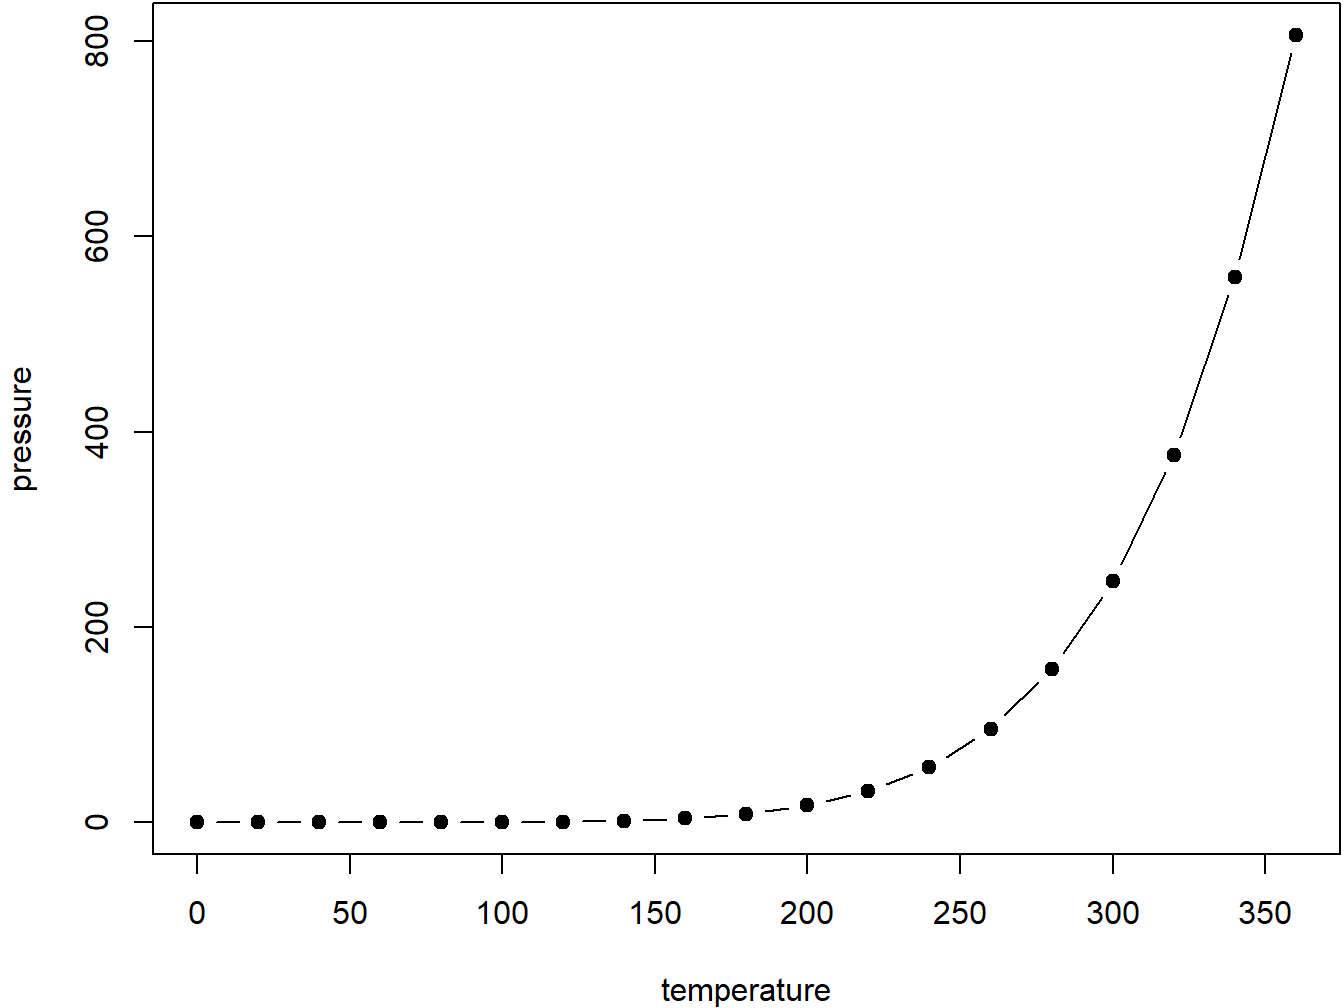
\includegraphics[width=0.8\linewidth]{01-intro_files/figure-latex/nice-fig-1} 

}

\caption{Here is a nice figure!}\label{fig:nice-fig}
\end{figure}

Reference a figure by its code chunk label with the \texttt{fig:} prefix, e.g., see Figure \ref{fig:nice-fig}. Similarly, you can reference tables generated from \texttt{knitr::kable()}, e.g., see Table \ref{tab:nice-tab}.

\begin{Shaded}
\begin{Highlighting}[]
\NormalTok{knitr}\SpecialCharTok{::}\FunctionTok{kable}\NormalTok{(}
  \FunctionTok{head}\NormalTok{(iris, }\DecValTok{20}\NormalTok{), }\AttributeTok{caption =} \StringTok{\textquotesingle{}Here is a nice table!\textquotesingle{}}\NormalTok{,}
  \AttributeTok{booktabs =} \ConstantTok{TRUE}
\NormalTok{)}
\end{Highlighting}
\end{Shaded}

\begin{table}

\caption{\label{tab:nice-tab}Here is a nice table!}
\centering
\begin{tabular}[t]{rrrrl}
\toprule
Sepal.Length & Sepal.Width & Petal.Length & Petal.Width & Species\\
\midrule
5.1 & 3.5 & 1.4 & 0.2 & setosa\\
4.9 & 3.0 & 1.4 & 0.2 & setosa\\
4.7 & 3.2 & 1.3 & 0.2 & setosa\\
4.6 & 3.1 & 1.5 & 0.2 & setosa\\
5.0 & 3.6 & 1.4 & 0.2 & setosa\\
\addlinespace
5.4 & 3.9 & 1.7 & 0.4 & setosa\\
4.6 & 3.4 & 1.4 & 0.3 & setosa\\
5.0 & 3.4 & 1.5 & 0.2 & setosa\\
4.4 & 2.9 & 1.4 & 0.2 & setosa\\
4.9 & 3.1 & 1.5 & 0.1 & setosa\\
\addlinespace
5.4 & 3.7 & 1.5 & 0.2 & setosa\\
4.8 & 3.4 & 1.6 & 0.2 & setosa\\
4.8 & 3.0 & 1.4 & 0.1 & setosa\\
4.3 & 3.0 & 1.1 & 0.1 & setosa\\
5.8 & 4.0 & 1.2 & 0.2 & setosa\\
\addlinespace
5.7 & 4.4 & 1.5 & 0.4 & setosa\\
5.4 & 3.9 & 1.3 & 0.4 & setosa\\
5.1 & 3.5 & 1.4 & 0.3 & setosa\\
5.7 & 3.8 & 1.7 & 0.3 & setosa\\
5.1 & 3.8 & 1.5 & 0.3 & setosa\\
\bottomrule
\end{tabular}
\end{table}

You can write citations, too. For example, we are using the \textbf{bookdown} package (\protect\hyperlink{ref-R-bookdown}{Xie 2020}) in this sample book, which was built on top of R Markdown and \textbf{knitr} (\protect\hyperlink{ref-xie2015}{Xie 2015}).

\hypertarget{U2}{%
\chapter{Comportamiento del Consumidor}\label{U2}}

La presente unidad ayudará a los estudiantes a comprender las decisiones económicas tomadas por los consumidores de alimentos y productos agrícolas. Los temas incluyen las fuerzas que influyen en el comportamiento del consumidor (Sección 3); el concepto de demanda de mercado para un producto en particular (Sección 4); y la elasticidad de la demanda (Sección 5). La especificación de medidas clave de elasticidad se complementa con ejemplos empíricos y su relevancia para la toma de decisiones en la industria de alimentos y fibras, incluida la magnitud potencial de la respuesta del consumidor y su implicancia en los ingresos del productor.

\hypertarget{Sec3}{%
\section*{Sección 3: Teoría del comportamiento del consumidor}\label{Sec3}}
\addcontentsline{toc}{section}{Sección 3: Teoría del comportamiento del consumidor}

El proceso biológico de la fotosíntesis, en el que la adición de luz al entorno de una planta da como resultado el crecimiento de esta, se puede considerar en un contexto de estímulo-respuesta. El estímulo es la adición de luz, y la respuesta es el crecimiento de la planta. Este proceso se puede estudiar en un entorno controlado utilizando sofisticados dispositivos de medición.

El comportamiento económico también se puede pensar en un contexto de estímulo-respuesta. Por ejemplo, una caída en el precio del helado actúa como un estímulo, provocando que los consumidores compren más helado. Estas compras se pueden medir y registrar.

En la mayoría de los aspectos, sin embargo, las similitudes terminan aquí. El complejo proceso de la fotosíntesis puede examinarse y estudiarse directamente, pero la mayoría de los procesos de comportamiento económico no pueden estudiarse de esta manera. De hecho, este ejemplo ilustra la distinción entre las ciencias naturales (por ejemplo, biología, química, física) y las ciencias sociales (por ejemplo, economía). La mayoría de los procesos de comportamiento económico no se pueden estudiar en un entorno controlado.

Podemos examinar las relaciones técnicas de conversión de insumos a productos en un proceso de producción, pero no podemos observar el proceso de conectar el estímulo económico con una decisión económica. ¿Por qué Juan compra más helado que Sofía cuando ambos enfrentan los mismos precios y tienen los mismos ingresos?

Las teorías económicas más prominentes sobre el comportamiento del consumidor asumen que los consumidores son racionales y buscan maximizar su satisfacción sin salirse de su presupuesto. En esta sección, discutimos la teoría del consumidor y cómo se puede utilizar para comprender el comportamiento de los consumidores.

\hypertarget{Sec4}{%
\section*{Sección 4: Equilibrio del Consumidor y Demanda del Mercado}\label{Sec4}}
\addcontentsline{toc}{section}{Sección 4: Equilibrio del Consumidor y Demanda del Mercado}

\hypertarget{Sec5}{%
\section*{Sección 5: Medidas e interpretación de elasticidades}\label{Sec5}}
\addcontentsline{toc}{section}{Sección 5: Medidas e interpretación de elasticidades}

Here is a review of existing methods.

\hypertarget{U3}{%
\chapter{Oferta y Mercado Agrario}\label{U3}}

\hypertarget{Sec6}{%
\section*{Sección 6: Introducción a la producción y el uso de Recursos}\label{Sec6}}
\addcontentsline{toc}{section}{Sección 6: Introducción a la producción y el uso de Recursos}

\hypertarget{Sec7}{%
\section*{Sección 7: Economía de los Factores de Producción y Sustitución de productos}\label{Sec7}}
\addcontentsline{toc}{section}{Sección 7: Economía de los Factores de Producción y Sustitución de productos}

\hypertarget{Sec8}{%
\section*{Sección 8: Equilibrio de Mercado y precio del producto: Competencia Perfecta}\label{Sec8}}
\addcontentsline{toc}{section}{Sección 8: Equilibrio de Mercado y precio del producto: Competencia Perfecta}

\hypertarget{Sec9}{%
\section*{Sección 9: Competencia Imperfecta: Equilibrio de Mercado y precios}\label{Sec9}}
\addcontentsline{toc}{section}{Sección 9: Competencia Imperfecta: Equilibrio de Mercado y precios}

We describe our methods in this chapter.

\hypertarget{U4}{%
\chapter{Rol del Gobierno en la Industria Agroalimentaria}\label{U4}}

\hypertarget{Sec10}{%
\section*{Sección 10: Recursos Naturales, Medioambiente y Agricultura}\label{Sec10}}
\addcontentsline{toc}{section}{Sección 10: Recursos Naturales, Medioambiente y Agricultura}

\hypertarget{Sec11}{%
\section*{Sección 11: Intervención Gubernamental}\label{Sec11}}
\addcontentsline{toc}{section}{Sección 11: Intervención Gubernamental}

\hypertarget{Sec12}{%
\section*{Sección 12: Comercio Agrícola y tipos de cambio}\label{Sec12}}
\addcontentsline{toc}{section}{Sección 12: Comercio Agrícola y tipos de cambio}

\hypertarget{final-words}{%
\chapter{Final Words}\label{final-words}}

We have finished a nice book.

\hypertarget{refs}{}
\begin{CSLReferences}{1}{0}
\leavevmode\hypertarget{ref-xie2015}{}%
Xie, Yihui. 2015. \emph{Dynamic Documents with {R} and Knitr}. 2nd ed. Boca Raton, Florida: Chapman; Hall/CRC. \url{http://yihui.name/knitr/}.

\leavevmode\hypertarget{ref-R-bookdown}{}%
---------. 2020. \emph{Bookdown: Authoring Books and Technical Documents with r Markdown}. \url{https://CRAN.R-project.org/package=bookdown}.

\end{CSLReferences}

\end{document}
